\vspace{-1mm}
\section{Experimental Setup}
\label{sec:experimental_setup}

In this section, we provide the details of the experimental setup, including the hardware and software components used in our experiments. We also describe the data collection process, the data cleaning and preprocessing steps, and the feature extraction techniques employed to prepare the data for model training and testing.

\subsection{Hardware Setup}

Due to time and budget constraints, we used a scaled-down version of the proposed system. Model vehicles were used to simulate the parked vehicles in a parking lot. Preliminary experiments were conducted to evaluate the feasibility of using other types of objects, such as cardboard boxes, to represent parked vehicles. However, these objects did not yield satisfactory results, as they did not produce the same level of multipath propagation as real vehicles. Therefore, we decided to use model vehicles for our experiments. Furthermore, the material of the model vehicles was chosen to be similar to that of real vehicles, as this would help in achieving better results. The model vehicles used in our experiments were 1:12 scale models of real vehicles that were made of a relatively realistic combination of plastic and metal. The model vehicles were placed on a table, and the transmitter and receiver were positioned at a fixed distance from each other on the sides of the row of parking spots. Since the the number of classes to be classified is equal to two to the power of the number of parking spots, we used three parking spots and three model vehicles to create a total of eight classes. As transmitter and receiver, we used two ESP32 microcontrollers, which are low-cost, low-power microcontrollers with built-in Wi-Fi capabilities. The ESP32 microcontrollers were programmed to send and receive Wi-Fi signals, allowing us to collect Channel State Information (CSI) data from the wireless signals. 

\begin{figure}[H]
    \begin{center}
        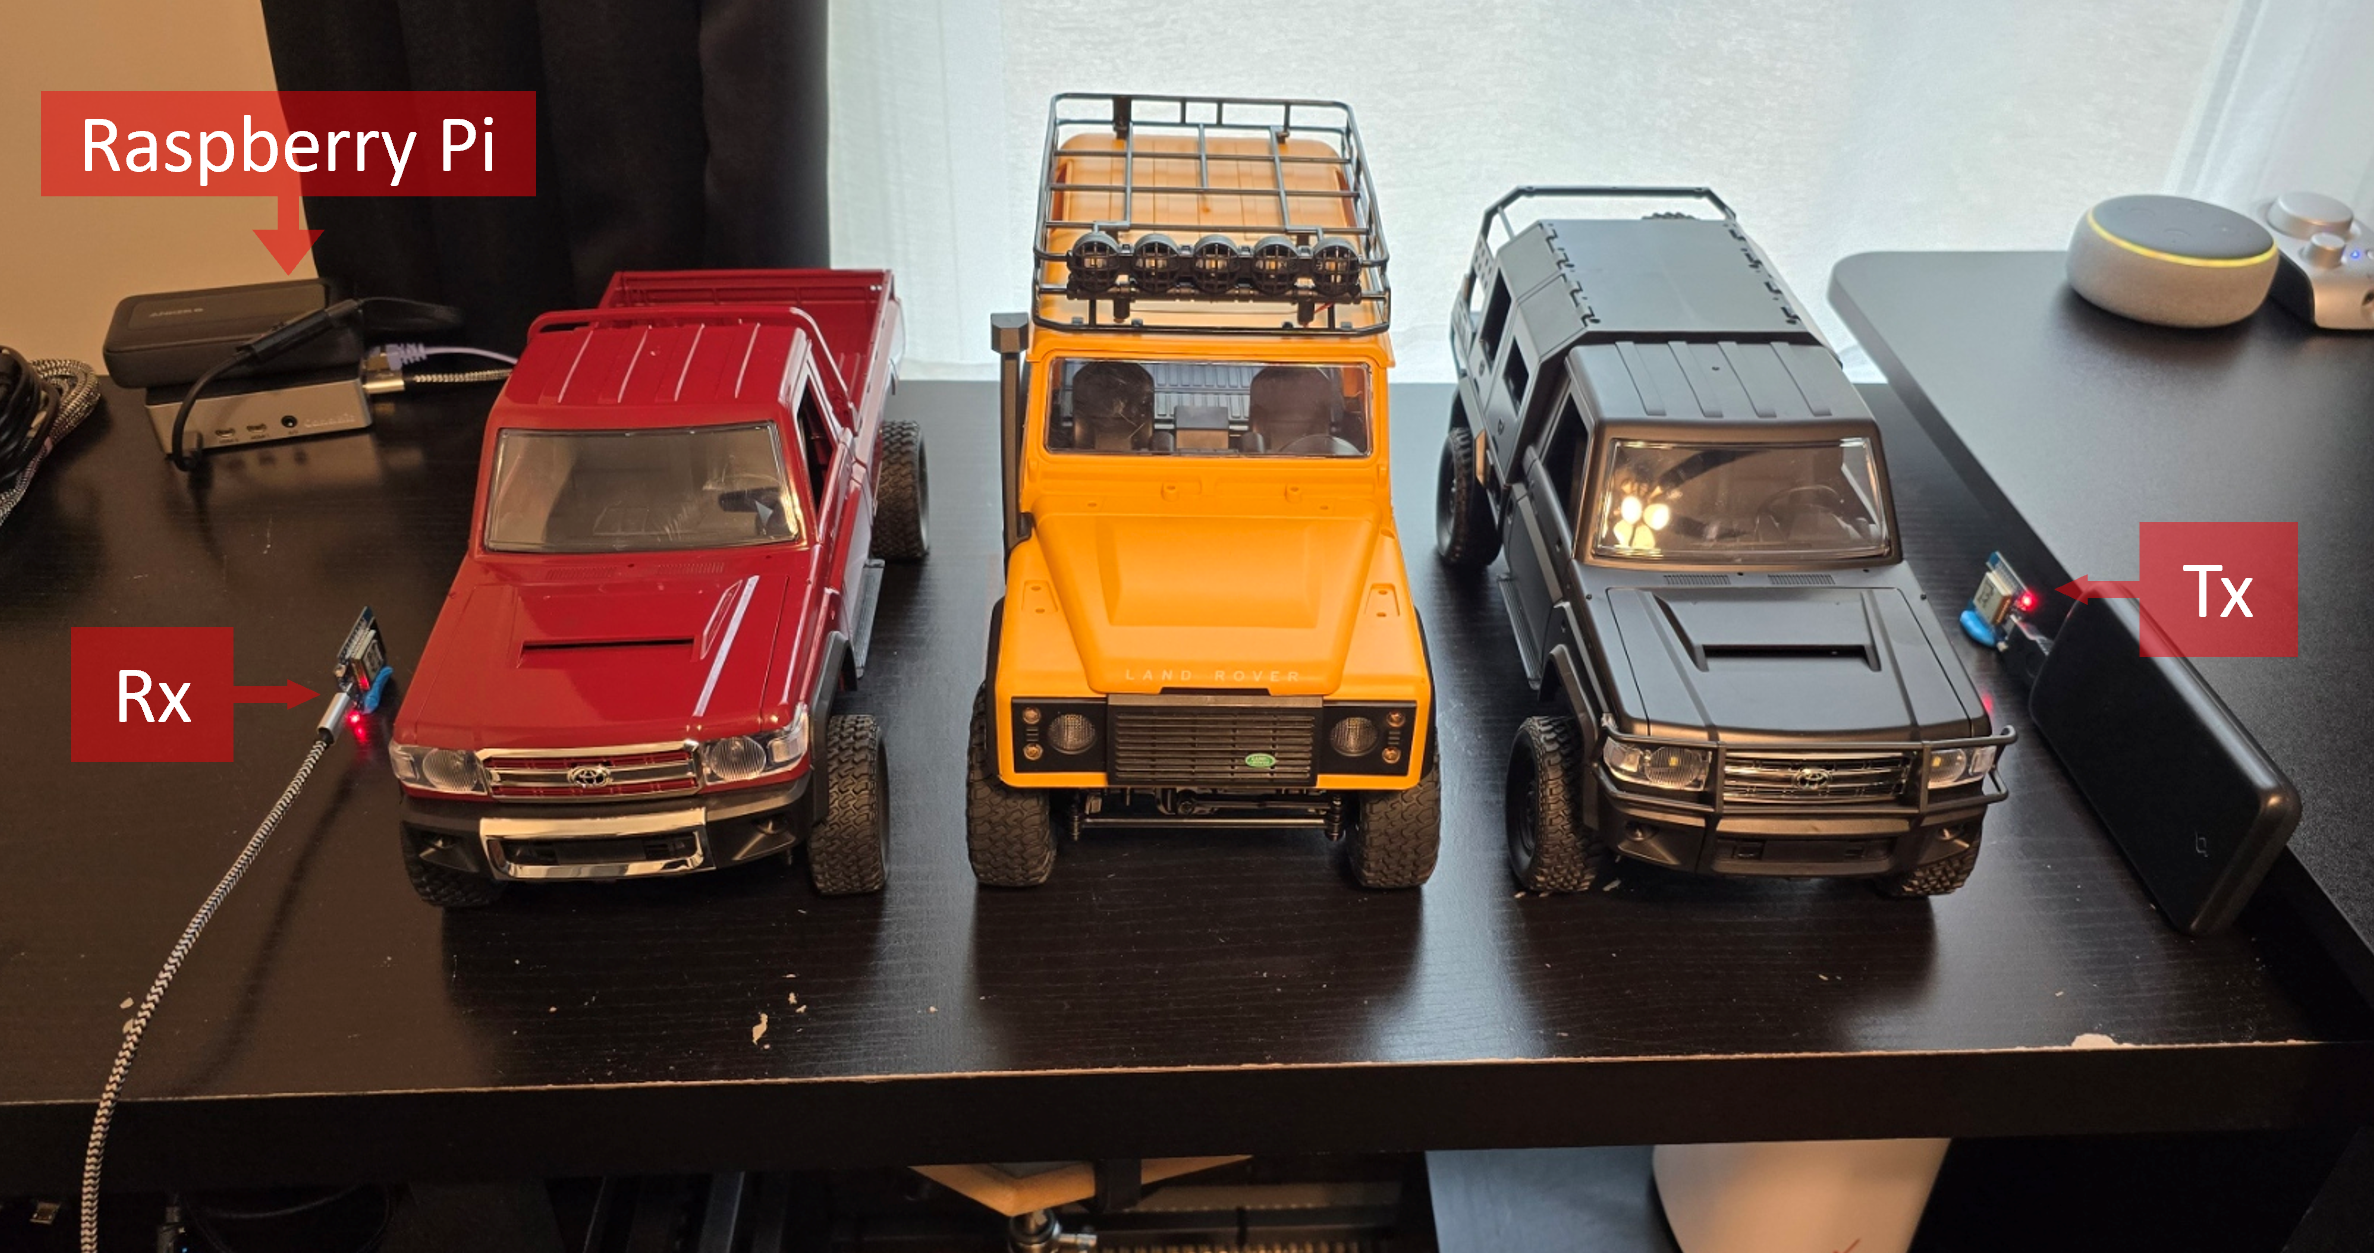
\includegraphics[width=8cm]{Figures/experimental_setup.png}\vspace{0mm}
        \caption{Experimental setup for data collection}\vspace{0mm}
        \label{fig:experimental_setup}
    \end{center}
\end{figure}

As shown in Figure~\ref{fig:experimental_setup}, the transmitter was placed on one side of the parking spots, while the receiver was placed on the other side. The transmitter was connected only to an off the shelf portable power bank, which emphasizes the low-cost and low-power nature of our system. The receiver was connected to a Raspberry Pi, which was used to store the collected data. For each parking combination, the CSI data was collected for 10 seconds, and this process was repeated 20 times.

\subsection{Software Setup}

The ESP32 microcontrollers were flashed with a custom firmware that enabled them to send and receive Wi-Fi signals. The firmware was based on a previous work that provided a framework for collecting CSI data from ESP32 devices\cite{9217780}. The resulting CSI data in a CSV format was then transferred to another computer for further processing. The data was cleaned by removing null values followed by a preprocessing step using a moving average filter to smooth out noise and fluctuations in the signal. In order to extract features from the raw CSI data,  amplitude and phase values were calculated for each subcarrier at each time instance. The amplitude and phase values were then used to create a feature vector for each data point. The data was then split into training and testing sets, with 80\% of the data used for training and 20\% for testing. The training set was used to train a machine learning model, while the testing set was used to evaluate the performance of the model. A Convolutional Neural Network (CNN) with 9 layers was used for the model training and testing. The CNN model was implemented using TensorFlow and Keras libraries in Python. The model was trained using the training set, and the performance of the model was evaluated using the testing set. A sliding window method was used to create the training and testing sets, where a window of size 50 was used to create overlapping segments of the data.